\documentclass{article}
\usepackage{graphicx} % Required for inserting images
\usepackage{tikz}
\usepackage{float}
\usepackage{url}
\usepackage{amsmath}
\usepackage{hyperref}
\usepackage{pgfplots}
\usetikzlibrary{positioning}
\pgfplotsset{compat=1.18}


\begin{document}

\begin{titlepage}
    \centering

    \noindent
    \begin{minipage}[t]{0.55\textwidth}
        \raggedright
        \includegraphics[height=1.6cm]{SG.png}\hspace{0.5em}%
    \end{minipage}%
    \hfill
    \begin{minipage}[t]{0.35\textwidth}
        \raggedleft
        \includegraphics[height=1.6cm]{mines.png}
    \end{minipage}

    \vspace{1cm}

    \noindent
    {\color{violetstage}\bfseries\large Benguedda --Lauzon Elias}\\[0.2em]

    \vspace{0.8cm}

    \noindent
    {\color{violetstage}\bfseries\scshape École nationale supérieure des mines de Saint-Étienne}\\[0.2em]
    {\color{violetstage}\bfseries 158 Cours Fauriel, 42023 Saint-Étienne cedex 2}

    \vspace{3cm}

    {\color{violetstage}\bfseries\Large Rapport de stage « Assistant-ingénieur »}\\[1em]
    {\color{violetstage}\bfseries\large Recherche Quantitative}\\[1.5em]
    {\color{violetstage}\bfseries\large Correlation Modelling}\\[1.5em]


    \vfill

    \begin{flushleft}
    {\color{violetstage}\bfseries Entreprise d'accueil :} Société Générale, Pricing Team, \\
    Adresse(s) : 15 Parvis de la Défense, 92800 Puteaux.\\[0.6em]
    {\color{violetstage}\bfseries Tuteur Entreprise :} KONE Lanzeni (Ingénieur Pricing)\\[0.6em]
    {\color{violetstage}\bfseries Enseignant référent :} RULLIERE Didier
    \end{flushleft}

\end{titlepage}



\tableofcontents



\clearpage

\section*{Acknowledgements}

I would like to express my sincere gratitude to all the people who contributed to making this experience both enriching and rewarding.

First, I would like to thank my supervisor, Kone L., for their guidance, availability, and valuable advice throughout this experience. Their support and feedback allowed me to progressively develop my skills and gain a better understanding of the professional environment.

I would also like to thank the members of the Pricing Team for their warm welcome, their support, and the time they dedicated to answering my questions and sharing their knowledge. Working alongside them was an important part of this experience and allowed me to discover new professional and technical perspectives.


Finally, I would like to thank everyone who, directly or indirectly, contributed to this experience and helped make it a valuable step in my academic and professional development.
\clearpage

\section{Description of the company}

Société Générale (SG) is one of the four major banking groups in France. It was founded in 1864 and is a banking group whose activities are divided into two groups retail banking and investment banking. The group is present internationally through offices all around the world and employs more than 100,000 people worldwide. Its turnover is around \$ 25 Billion per year. 

Société Générale Securities Servicies (SGSS) is a subsidiary of the Société Générale Group specialized in securities services and providing solutions to financial institutions. Its activities are part of what we call in bank middle and front office activities.

My internship took place within SGSS in the Pricing Team desk. The team provides pricing services to various financial institutions, including BBVA, Goldman Sachs, J.P. Morgan, and CNP. This pricing activity is a part of the regulatory requirement imposed by the french regulator: the AMF (Autorité des Marchés Financiers) which aims to provide clarity and to ensure transparency of financial products to avoid financial crisis.

The team in which I worked is called Pricing Team. Its main role is therefore to value structured products and OTC derivatives with a quantitative approach. This activity lies at the intersection of quantitative tools and client relationship.



\section{Definition of the objectives}

During my internship, I had the opportunity to work on two projects involving two very different types of financial assets. The first project focused on interest rate securities (callable bonds, presented in a separate report), and the second one was about equity assets. This report is dedicated to the second project: correlation modelling.

\subsection{Correlation}

The second project of my internship focused on the pricing of derivatives based on two underlying assets, named Worst Of (WO) and Best Of (BO) products. In order to price these products accurately, it is necessary to model the dependence between the two underlying assets. This is where correlation plays a key role.

Here is an example of what a dataset can look like.

\begin{figure}[H]
    \centering
    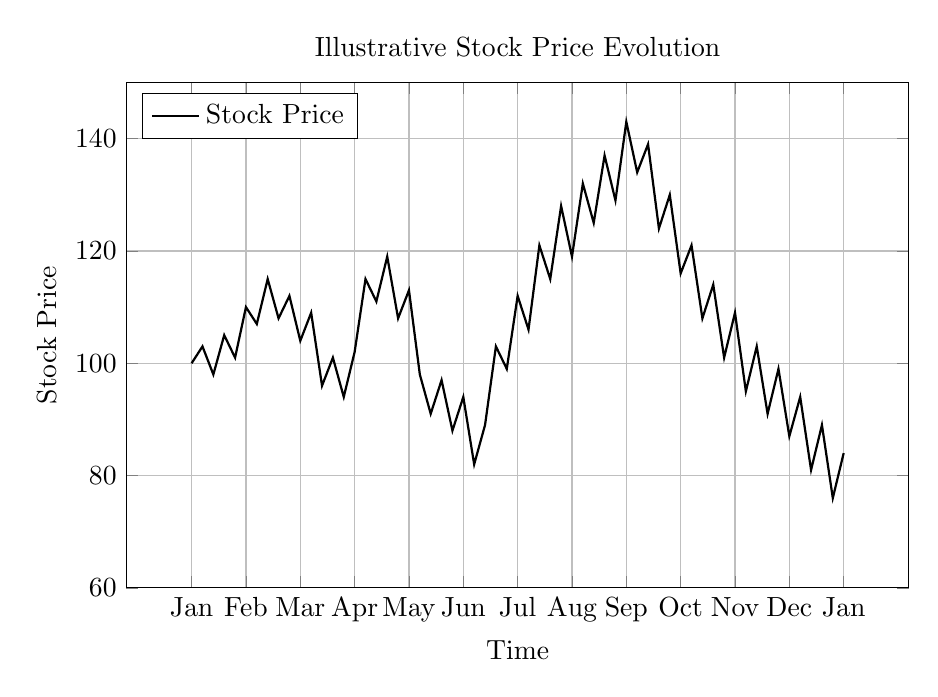
\begin{tikzpicture}
        \begin{axis}[
            width=0.95\textwidth,
            height=8cm,
            xlabel={Time},
            ylabel={Stock Price},
            title={Illustrative Stock Price Evolution},
            grid=major,
            minor grid style={draw=none},
            xtick={0,5,10,15,20,25,30,35,40,45,50,55,60},
            xticklabels={
                Jan,Feb,Mar,Apr,May,Jun,Jul,Aug,Sep,Oct,Nov,Dec,Jan
            },
            ymin=60,
            ymax=150,
            legend style={
                at={(0.02,0.98)},
                anchor=north west
            }
        ]

        \addplot[
            thick
        ] coordinates {
            (0,100)
            (1,103)
            (2,98)
            (3,105)
            (4,101)
            (5,110)
            (6,107)
            (7,115)
            (8,108)
            (9,112)
            (10,104)
            (11,109)
            (12,96)
            (13,101)
            (14,94)
            (15,102)
            (16,115)
            (17,111)
            (18,119)
            (19,108)
            (20,113)
            (21,98)
            (22,91)
            (23,97)
            (24,88)
            (25,94)
            (26,82)
            (27,89)
            (28,103)
            (29,99)
            (30,112)
            (31,106)
            (32,121)
            (33,115)
            (34,128)
            (35,119)
            (36,132)
            (37,125)
            (38,137)
            (39,129)
            (40,143)
            (41,134)
            (42,139)
            (43,124)
            (44,130)
            (45,116)
            (46,121)
            (47,108)
            (48,114)
            (49,101)
            (50,109)
            (51,95)
            (52,103)
            (53,91)
            (54,99)
            (55,87)
            (56,94)
            (57,81)
            (58,89)
            (59,76)
            (60,84)
        };

        \addlegendentry{Stock Price}

        \end{axis}
    \end{tikzpicture}
    \caption{Illustrative example of an erratic stock price evolution over time.}
    \label{fig:erratic_stock}
\end{figure}



To illustrate this concept, consider a basket composed of two stocks, Kering (KER) and LVMH (MC). Both companies operate in the luxury goods sector and are listed on the Paris stock exchange. Since they belong to the same industry and can be affected by similar economic factors, their stock prices tend to exhibit a relatively strong positive correlation over time. As a simplified historical example, their correlation can be considered to be around $0.7$. In contrast, consider a basket composed of Kering (KER) and Société Générale (GLE). These two companies operate in very different sectors and are therefore generally less dependent on the same economic factors. Their historical correlation is consequently much lower, with an absolute value closer to $0.2$.

A Worst Of or Best Of product is a structured product whose payoff at maturity depends on the performance of the least or best performing asset in a basket. For a basket composed of two assets, the payoff is therefore determined by the minimum or maximum performance of the two underlying assets. For example, in a simplified setting, the payoff of a Worst Of product can be expressed as

\begin{equation}
\text{Payoff}_{WO}(T)
=
\min\left(S_1(T),S_2(T)\right),
\end{equation}

while the payoff of a Best Of product can be expressed as

\begin{equation}
\text{Payoff}_{BO}(T)
=
\max\left(S_1(T),S_2(T)\right),
\end{equation}

\\

where $S_1(T)$ and $S_2(T)$ denote the values of the two underlying assets at maturity $T$. In practice, the payoff can also depend on the initial prices, strike levels, barriers, coupons, or other contractual features specified in the term sheet.

The importance of correlation can be understood intuitively by considering the two extreme cases. If the two assets are perfectly positively correlated, with a correlation equal to $1$, they tend to move in the same direction. Their performances are therefore relatively close to each other, which reduces the dispersion between the best and worst performers. Conversely, if the two assets are negatively correlated, their performances tend to move in opposite directions. This increases the dispersion between the two assets and therefore has a significant impact on the value of both Worst Of and Best Of products.

Consequently, correlation is a key input for the pricing of these products. A change in the assumed correlation can significantly modify the expected payoff and therefore the theoretical price of the structured product. The Pricing Team therefore needed a methodology to estimate and model the correlation between the underlying assets in order to incorporate this parameter into the pricing models.

The objective of my second project was therefore to study and model the correlation between two financial assets. The work involved analysing historical market data, estimating the dependence between the two underlying assets, and determining an appropriate correlation parameter for use in the pricing of Worst Of and Best Of products.



% ============================================================
% Correlation illustration
% ============================================================

\begin{figure}[H]
    \centering

    % --------------------------------------------------------
    % KER vs MC
    % --------------------------------------------------------
    \begin{minipage}{0.48\textwidth}
        \centering

        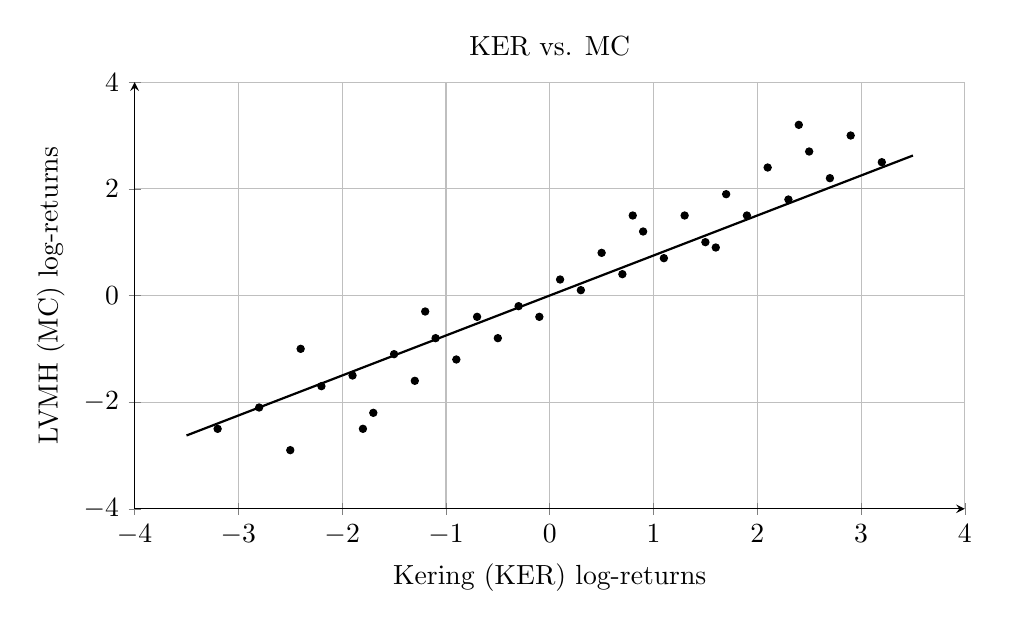
\begin{tikzpicture}
            \begin{axis}[
                width=\textwidth,
                height=7cm,
                xlabel={Kering (KER) log-returns},
                ylabel={LVMH (MC) log-returns},
                title={KER vs. MC},
                grid=major,
                xmin=-4, xmax=4,
                ymin=-4, ymax=4,
                axis lines=left
            ]

            \addplot[
                only marks,
                mark=*,
                mark size=1.3pt
            ] coordinates {
                (-3.2,-2.5)
                (-2.8,-2.1)
                (-2.5,-2.9)
                (-2.2,-1.7)
                (-1.9,-1.5)
                (-1.7,-2.2)
                (-1.5,-1.1)
                (-1.3,-1.6)
                (-1.1,-0.8)
                (-0.9,-1.2)
                (-0.7,-0.4)
                (-0.5,-0.8)
                (-0.3,-0.2)
                (-0.1,-0.4)
                (0.1,0.3)
                (0.3,0.1)
                (0.5,0.8)
                (0.7,0.4)
                (0.9,1.2)
                (1.1,0.7)
                (1.3,1.5)
                (1.5,1.0)
                (1.7,1.9)
                (1.9,1.5)
                (2.1,2.4)
                (2.3,1.8)
                (2.5,2.7)
                (2.7,2.2)
                (2.9,3.0)
                (3.2,2.5)
                (-2.4,-1.0)
                (-1.8,-2.5)
                (-1.2,-0.3)
                (0.8,1.5)
                (1.6,0.9)
                (2.4,3.2)
            };

            % Approximate regression line
            \addplot[
                thick,
                domain=-3.5:3.5
            ] {0.75*x};

        \end{axis}
        \end{tikzpicture}

        \vspace{0.2cm}

        \centering
        $\rho_{KER,MC} \approx 0.7$

    \end{minipage}
    \hfill
    % --------------------------------------------------------
    % KER vs GLE
    % --------------------------------------------------------
    \begin{minipage}{0.48\textwidth}
        \centering

        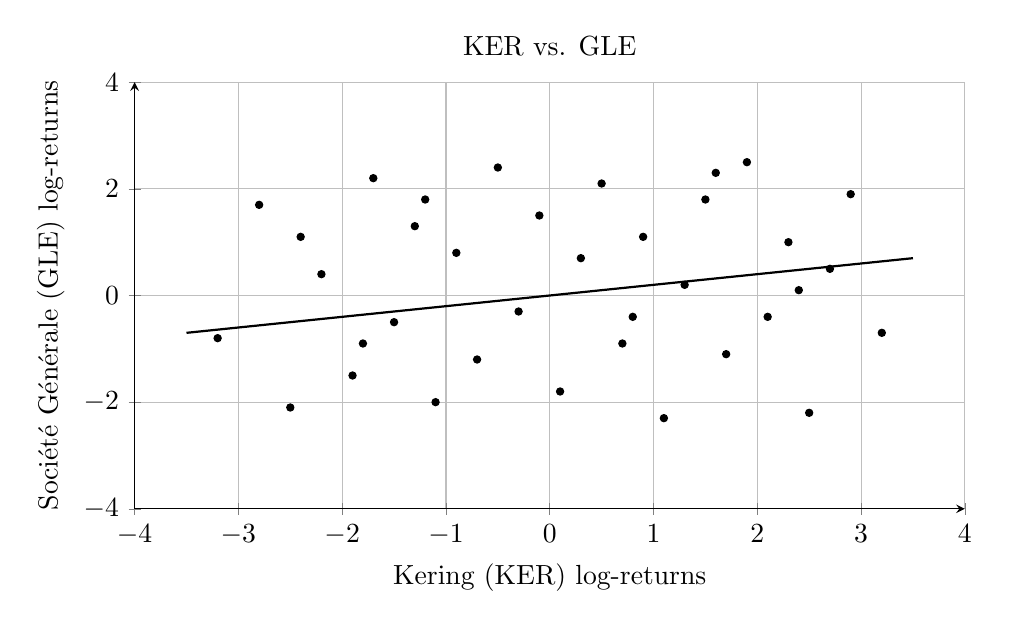
\begin{tikzpicture}
            \begin{axis}[
                width=\textwidth,
                height=7cm,
                xlabel={Kering (KER) log-returns},
                ylabel={Société Générale (GLE) log-returns},
                title={KER vs. GLE},
                grid=major,
                xmin=-4, xmax=4,
                ymin=-4, ymax=4,
                axis lines=left
            ]

            \addplot[
                only marks,
                mark=*,
                mark size=1.3pt
            ] coordinates {
                (-3.2,-0.8)
                (-2.8,1.7)
                (-2.5,-2.1)
                (-2.2,0.4)
                (-1.9,-1.5)
                (-1.7,2.2)
                (-1.5,-0.5)
                (-1.3,1.3)
                (-1.1,-2.0)
                (-0.9,0.8)
                (-0.7,-1.2)
                (-0.5,2.4)
                (-0.3,-0.3)
                (-0.1,1.5)
                (0.1,-1.8)
                (0.3,0.7)
                (0.5,2.1)
                (0.7,-0.9)
                (0.9,1.1)
                (1.1,-2.3)
                (1.3,0.2)
                (1.5,1.8)
                (1.7,-1.1)
                (1.9,2.5)
                (2.1,-0.4)
                (2.3,1.0)
                (2.5,-2.2)
                (2.7,0.5)
                (2.9,1.9)
                (3.2,-0.7)
                (-2.4,1.1)
                (-1.8,-0.9)
                (-1.2,1.8)
                (0.8,-0.4)
                (1.6,2.3)
                (2.4,0.1)
            };

            % Approximate regression line
            \addplot[
                thick,
                domain=-3.5:3.5
            ] {0.2*x};

        \end{axis}
        \end{tikzpicture}

        \vspace{0.2cm}

        \centering
        $\rho_{KER,GLE} \approx 0.2$

    \end{minipage}

    \caption{Illustration of the difference in correlation between Kering and LVMH, and between Kering and Société Générale. The simulated returns illustrate the stronger positive dependence between companies operating in the same sector.}
    \label{fig:correlation_illustration}

\end{figure}


\clearpage
\section{Correlation Modelling}

As said before we aim to price Worst of and Best of product. Correlation is the most useful feature that we need to approximate in order to price accurately these assets. Since correlations are not necessarily constant over time, several approaches are used by the market participants as a simple historical correlation  to dynamic econometric and machine learning models.

Let $S_t^i$ denote the closing price of asset $i$ at time $t$. The logarithmic return of price is defined as:

\begin{equation}
r_t^i
=
\ln\left(
\frac{S_t^i}{S_{t-1}^i}
\right).
\end{equation}

For $N$ assets, the return vector is

\begin{equation}
\bm{r}_t
=
\left(
r_t^1,\ldots,r_t^N
\right)^\top,
\end{equation}

and the correlation matrix is denoted by

\begin{equation}
\mathbf{R}_t
=
\left[
\rho_{ij,t}
\right]_{i,j=1,\ldots,N}.
\end{equation}

During the internship in order to reduce the noise of the data we will use the 5-days log-return :

\begin{equation}
r_t^i
=
\ln\left(
\frac{S_t^i}{S_{t-5}^i}
\right).
\end{equation}

This measure permits to have a weekly log return\footnote{European and American markets are open from monday to friday}.

Please note that because data is expansive and strictly confidential, for the purpose of this paper, we won't be able to disclose exact values but only estimations.

As we used to proceed, we will create two different samples, One for test and the other one for training, we will use 80\% of the data for training and 20\% for test.

Our benchmark are the price of Worst Of and Best Of assets which are sometimes quoted on by market on Bloomberg \footnote{https://www.bloomberg.com}. 

\subsection{Correlation Models}

We next present the models that we use to estimate the correlation between assets.

We also have another method that is striclty confidential from ICE \footnote{https://www.ice.com/fixed-income-data-services/data-and-analytics/exchange-data}, which is a data provider. It will be useful to compare our estimation with the data provided by ICE.

% ============================================================
\subsubsection{Constant Historical Correlation}
% ============================================================

The first model that we have worked in is constant correlation. Even if at first sight this model is too simple it presents the advantage of being reproducible because completely reproducible during simulation. Actually, this little condition is really important for AMF because it allows the pricing team to always give the same price to the customer if the inputs don't change. Because providers of data are sometimes wrong, the Pricing Team often needs to recalculate the price of their structured products and then need the same correlation as before. This point leads us to really consider this method more than a stochastic method at first. 

The historical correlation model assumes that the dependence structure remains constant over the estimation period. For two assets $i$ and $j$, the Pearson correlation is

\begin{equation}
\hat{\rho}_{ij}
=
\frac{
\sum_{t=1}^{T}
(r_t^i-\bar r^i)(r_t^j-\bar r^j)
}{
\sqrt{
\sum_{t=1}^{T}(r_t^i-\bar r^i)^2
}
\sqrt{
\sum_{t=1}^{T}(r_t^j-\bar r^j)^2
}
},
\end{equation}

where $\bar r^i$ and $\bar r^j$ are the sample mean returns.

The historical correlation matrix is therefore

\begin{equation}
\mathbf{R}^{Hist}
=
\left[
\hat{\rho}_{ij}
\right]_{i,j=1,\ldots,N}.
\end{equation}

However, even if this method seem to be simple to put in place, we are facing multiple issues for example, we don't know what is the window we need to consider to calculate the correlation or the weight we should put to each observation.

% ============================================================
\subsubsection{EWMA Correlation}
% ============================================================

The Exponentially Weighted Moving Average (EWMA) model introduces time variation by assigning a larger weight to recent observations. The covariance matrix is recursively 
defined as

\begin{equation}
\mathbf{\Sigma}_t^{EWMA}
=
\lambda\mathbf{\Sigma}_{t-1}^{EWMA}
+
(1-\lambda)
\bm{r}_{t-1}\bm{r}_{t-1}^{\top},
\end{equation}

where $\lambda\in[0,1]$ is the decay factor. The parameter $\lambda$ is a hyper parameter of the model and has been optimized using the market data.

The conditional correlation matrix is obtained by normalizing the covariance matrix:

\begin{equation}
\mathbf{R}_t^{EWMA}
=
\mathbf{D}_t^{-1/2}
\mathbf{\Sigma}_t^{EWMA}
\mathbf{D}_t^{-1/2},
\end{equation}

with

\begin{equation}
\mathbf{D}_t
=
\operatorname{diag}
\left(
\Sigma_{11,t}^{EWMA},
\ldots,
\Sigma_{NN,t}^{EWMA}
\right).
\end{equation}

For two assets, this gives

\begin{equation}
\rho_{ij,t}^{EWMA}
=
\frac{
\Sigma_{ij,t}^{EWMA}
}{
\sqrt{
\Sigma_{ii,t}^{EWMA}
\Sigma_{jj,t}^{EWMA}
}
}.
\end{equation}

This model has been proposed by the Pricing Team as the first sophisticated model to explore, and I worked on it using the J.P. Morgan paper \cite{JP Morgan EWMA}

This model has the benefit to also be reproducible as soon as there isn't any stochasticity. It also permits to give more importance to certain observations

We also finally get a lambda close to 0.93 that permits to have great approximation to the correlation given by the market when we compare our price with the ones observed on the market on thi type of asset.


% ============================================================
\subsubsection{DCC-GARCH}
% ============================================================

The DCC-GARCH model was considered in order to capture the
time-varying dependence between the two underlying assets. Unlike the
simple historical correlation method we have done first, the DCC-GARCH model allows the correlation to evolve over time according to the information contained in recent market returns.

The model was estimated using historical return data over an observation period of several years. For confidentiality reasons, the exact estimation period and numerical results are not disclosed in this report. The values presented below are therefore illustrative and are intended only to describe the methodology and the type of results obtained.

The individual volatility dynamics were first modelled using a GARCH(1,1) specification:

\begin{equation}
\sigma_{i,t}^{2}
=
\omega_i
+
\alpha_i r_{i,t-1}^{2}
+
\beta_i\sigma_{i,t-1}^{2}.
\end{equation}

The resulting standardised residuals were then used to estimate the
dynamic correlation parameters. In an illustrative calibration, the
estimated DCC parameters were found to be of the following order of
magnitude:

\begin{equation}
\alpha \approx 0.04,
\qquad
\beta \approx 0.93.
\end{equation}

These values illustrate a relatively persistent correlation process.
In particular, the relatively large value of $\beta$ indicates that
the correlation tends to remain close to its previous level, while
$\alpha$ determines the sensitivity of the correlation to new market
information.

The resulting dynamic correlation is represented in
Figure~\ref{fig:dcc_correlation}. The estimated correlation fluctuates
over time rather than remaining constant. For illustration, the
correlation can be considered to vary approximately between $0.45$
and $0.80$, with an average level around $0.65$.

\begin{figure}[H]
    \centering
    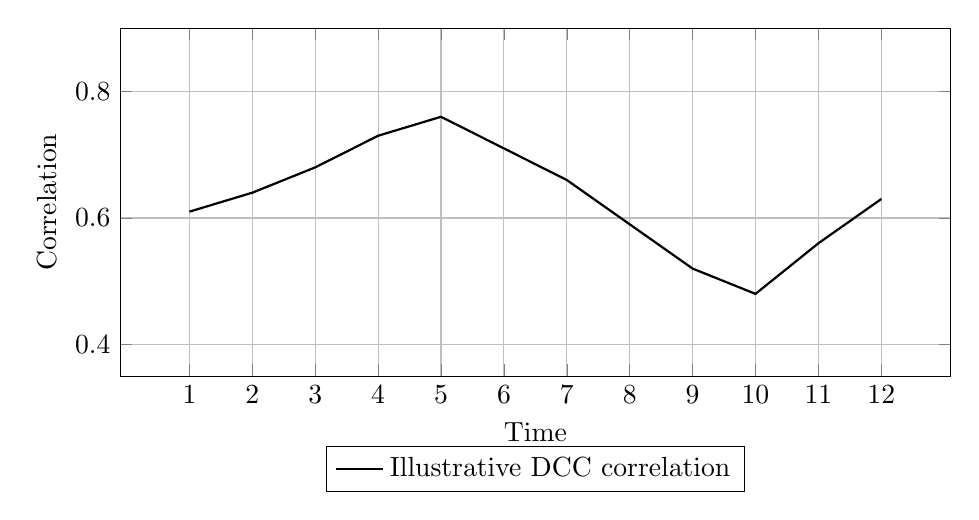
\begin{tikzpicture}
        \begin{axis}[
            width=\linewidth,
            height=6cm,
            xlabel={Time},
            ylabel={Correlation},
            ymin=0.35,
            ymax=0.90,
            grid=major,
            xtick={1,2,3,4,5,6,7,8,9,10,11,12},
            xticklabels={
                1,2,3,4,5,6,7,8,9,10,11,12
            },
            legend style={
                at={(0.5,-0.20)},
                anchor=north
            }
        ]
        \addplot[
            thick
        ] coordinates {
            (1,0.61)
            (2,0.64)
            (3,0.68)
            (4,0.73)
            (5,0.76)
            (6,0.71)
            (7,0.66)
            (8,0.59)
            (9,0.52)
            (10,0.48)
            (11,0.56)
            (12,0.63)
        };
        \addlegendentry{Illustrative DCC correlation}
        \end{axis}
    \end{tikzpicture}
    \caption{
        Illustrative dynamic correlation estimated using a DCC-GARCH
        model. Exact numerical results are not disclosed for
        confidentiality reasons.
    }
    \label{fig:dcc_correlation}
\end{figure}

Several periods of variation can be observed in the estimated
correlation. In particular, the correlation increases during periods
in which the two assets tend to react more strongly to common market
factors. Conversely, it decreases when their individual dynamics
become less synchronized.

The main advantage of the DCC-GARCH approach is therefore that it
does not impose a constant correlation throughout the observation
period. This is particularly relevant for Worst Of and Best Of
products, whose valuation depends on the joint behaviour of their
underlying assets.

However, the model also has several limitations. First, the estimated
correlation remains strongly dependent on the historical sample used
for calibration. Changing the observation window may therefore lead
to different estimates. Second, the model is essentially
backward-looking, since its parameters are inferred from historical
returns. Finally, the DCC specification imposes a particular dynamic
structure on the correlation and may not fully capture abrupt changes
in dependence during periods of financial stress.

For these reasons, the DCC-GARCH model was used as one possible
approach to describe the historical dynamics of correlation rather
than as a definitive representation of future dependence.

% ============================================================
\subsubsection{Ornstein--Uhlenbeck Model}
% ============================================================

The Ornstein--Uhlenbeck (OU) model was considered as an alternative
approach for modelling the time-varying dependence between the two
underlying assets. Its main characteristic is its mean-reverting
behaviour: when the process moves away from its long-term equilibrium
level, a deterministic force tends to bring it back towards this
level.  Effectively, when we look to the data there are periods when we can see a large decrease of correlation and right after it, we observe a mean reverting phenomenon.

Let $X_t$ denote a latent dependence factor. The Ornstein--Uhlenbeck
process is defined by the stochastic differential equation

\begin{equation}
dX_t
=
\kappa(\theta-X_t)\,dt
+
\sigma\,dW_t,
\end{equation}

where $\theta$ represents the constant of long-term mean level of the process,
$\kappa>0$ is the mean-reversion speed, $\sigma>0$ is the volatility
parameter, and $W_t$ is a standard Brownian motion.

The dynamics of the process can be separated into two components.
The first one,

\begin{equation}
\kappa(\theta-X_t)\,dt,
\end{equation}

is the deterministic mean-reverting component. Its sign depends on
the position of $X_t$ relative to $\theta$. If $X_t<\theta$, then

\begin{equation}
\kappa(\theta-X_t)>0,
\end{equation}

and the process is pushed upwards towards $\theta$. Conversely, if
$X_t>\theta$, then

\begin{equation}
\kappa(\theta-X_t)<0,
\end{equation}

and the process is pushed downwards. The parameter $\kappa$ therefore
controls the strength of the mean-reversion effect.

The second component,

\begin{equation}
\sigma\,dW_t,
\end{equation}

introduces random fluctuations around the long-term level. The
parameter $\sigma$ controls the magnitude of these fluctuations. In fact as we can see this model introduces a stochasticity process and is then not reproducible.  
\\

The OU process is a linear stochastic differential equation and admits
an explicit solution. Starting from an initial value $X_t$, we had to write while we were discretazing at $t+\Delta t$ :

\begin{equation}
X_{t+\Delta t}
=
\theta
+
(X_t-\theta)e^{-\kappa\Delta t}
+
\sigma
\int_t^{t+\Delta t}
e^{-\kappa(t+\Delta t-s)}
\,dW_s.
\end{equation}

The factor

\begin{equation}
e^{-\kappa\Delta t}
\end{equation}

is particularly important. It permitted to determine how much of the current deviation $(X_t-\theta)$ remains after a time interval $\Delta t$. Since $\kappa>0$, this factor decreases towards zero as time increases. Consequently, the influence of the initial value gradually disappears and the process tends to return towards $\theta$.

The stochastic integral is normally distributed with mean zero and
variance

\begin{equation}
\operatorname{Var}
\left(
\sigma
\int_t^{t+\Delta t}
e^{-\kappa(t+\Delta t-s)}
\,dW_s
\right)
=
\sigma^2
\frac{1-e^{-2\kappa\Delta t}}{2\kappa}.
\end{equation}

Therefore, the conditional distribution of $X_{t+\Delta t}$ given
$X_t$ is Gaussian:

\begin{equation}
X_{t+\Delta t}\mid X_t
\sim
\mathcal{N}
\left(
\theta+(X_t-\theta)e^{-\kappa\Delta t},
\,
\frac{\sigma^2}{2\kappa}
\left(1-e^{-2\kappa\Delta t}\right)
\right).
\end{equation}

This property was particularly useful fwhen we were calibrating the model during the simulations, since the process can be generated directly at discrete observation dates.

Introducing a standard normal random variable
$\varepsilon_t\sim\mathcal{N}(0,1)$, the exact discrete-time
representation is therefore

\begin{equation}
\boxed{
X_{t+\Delta t}
=
\theta
+
(X_t-\theta)e^{-\kappa\Delta t}
+
\sigma
\sqrt{
\frac{1-e^{-2\kappa\Delta t}}{2\kappa}
}
\,\varepsilon_t
}
\end{equation}

This equation was the one used to simulate the evolution of the
latent dependence factor.

\paragraph{Stationary Behaviour}

Another important property of the OU process is its stationary
distribution. When the process has been running for a sufficiently
long period, the influence of the initial value becomes negligible.
Indeed,

\begin{equation}
\lim_{\Delta t\rightarrow\infty}
e^{-\kappa\Delta t}
=
0.
\end{equation}

Consequently, the conditional mean converges towards $\theta$:

\begin{equation}
\lim_{\Delta t\rightarrow\infty}
\mathbb{E}[X_{t+\Delta t}\mid X_t]
=
\theta.
\end{equation}

The corresponding stationary variance is

\begin{equation}
\operatorname{Var}(X_t)
=
\frac{\sigma^2}{2\kappa}.
\end{equation}

Hence, the parameter $\kappa$ and the volatility $\sigma$ jointly
determine the long-run dispersion of the process.

The characteristic time scale of the mean reversion can also be
related to $\kappa$. A commonly used quantity is the half-life,
defined as the time required for the initial deviation from the
equilibrium level to be reduced by one half. Since

\begin{equation}
e^{-\kappa t_{1/2}}=\frac{1}{2},
\end{equation}

the half-life is given by

\begin{equation}
\boxed{
t_{1/2}
=
\frac{\ln(2)}{\kappa}
}
\end{equation}

This provides an intuitive interpretation of the mean-reversion
parameter. A large $\kappa$ corresponds to a short half-life and
therefore a rapid return towards the equilibrium level, whereas a
small $\kappa$ corresponds to a slower adjustment.


Unfortunately, the OU process itself cannot directly represent a correlation coefficient because $X_t$ takes reel values, whereas a correlation must satisfy

\begin{equation}
-1\leq\rho_t\leq1.
\end{equation}

To solve this problem, the latent factor is transformed using the
hyperbolic tangent function \footnote{\url{https://en.wikipedia.org/wiki/Fisher_transformation}}


This transformation also provides an intuitive interpretation of the
latent variable. Applying the inverse transformation gives

\begin{equation}
X_t
=
\operatorname{arctanh}(\rho_t)
=
\frac{1}{2}
\ln
\left(
\frac{1+\rho_t}{1-\rho_t}
\right).
\end{equation}

Thus, the OU process can be interpreted as a mean-reverting model for
the transformed correlation rather than for the correlation itself.

The long-term level of the correlation is obtained by applying the
same transformation to the equilibrium level $\theta$:

\begin{equation}
\boxed{
\rho_{\infty}
=
\tanh(\theta)
}
\end{equation}

\paragraph{Illustrative Dynamics}

The following figure illustrates the type of dynamics produced by the
model. The correlation fluctuates around a long-term level while
temporary deviations are gradually reduced by the mean-reversion
mechanism.

\begin{figure}[H]
    \centering
    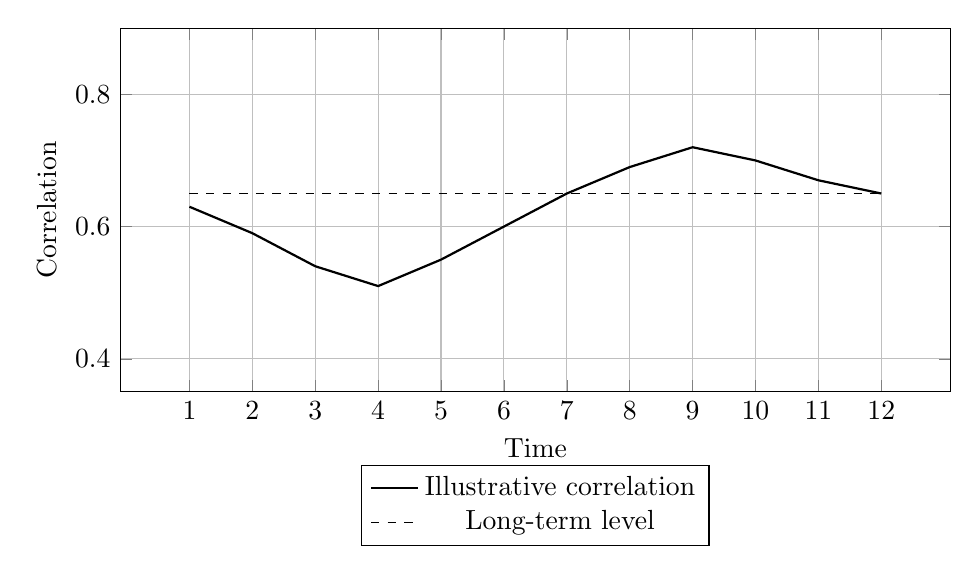
\begin{tikzpicture}
        \begin{axis}[
            width=\linewidth,
            height=6.2cm,
            xlabel={Time},
            ylabel={Correlation},
            ymin=0.35,
            ymax=0.90,
            grid=major,
            xtick={1,2,3,4,5,6,7,8,9,10,11,12},
            xticklabels={
                1,2,3,4,5,6,7,8,9,10,11,12
            },
            legend style={
                at={(0.5,-0.20)},
                anchor=north
            }
        ]

        \addplot[
            thick
        ] coordinates {
            (1,0.63)
            (2,0.59)
            (3,0.54)
            (4,0.51)
            (5,0.55)
            (6,0.60)
            (7,0.65)
            (8,0.69)
            (9,0.72)
            (10,0.70)
            (11,0.67)
            (12,0.65)
        };

        \addplot[
            dashed
        ] coordinates {
            (1,0.65)
            (12,0.65)
        };

        \addlegendentry{Illustrative correlation}
        \addlegendentry{Long-term level}

        \end{axis}
    \end{tikzpicture}

    \caption{
        Illustrative dynamics of the correlation generated by the
        Ornstein--Uhlenbeck model. The values are approximate and do
        not represent the confidential calibration results.
    }
    \label{fig:ou_correlation}
\end{figure}


The OU model therefore provides a relatively simple way of generating
a time-dependent correlation while preserving the required bounds
through the $\tanh$ transformation. The resulting process $\rho_t$
can subsequently be introduced into the correlation matrix used for
the Monte Carlo simulation of the two underlying assets.

In particular, at each simulation time step, the correlation matrix
takes the form

\begin{equation}
\mathbf{R}_t
=
\begin{pmatrix}
1 & \rho_t\\
\rho_t & 1
\end{pmatrix}.
\end{equation}

The evolution of $\rho_t$ therefore directly affects the dependence
between the simulated returns of the two assets. The OU model can
consequently be incorporated into the Monte Carlo framework used to
price the Worst Of and Best Of products.


The model provides a useful alternative to the DCC-GARCH approach and allows the sensitivity of the structured product using stochasticity and noise.


\subsection{Comparison of the Models}

The different correlation models considered during the internship had their own advantages and disadvantages.

The Historical model is the simplest approach and is assumed to be the first benchmarck. It is easy to implement and reproduce and permitted to get a first idea of the correlation between two assets, but it does not capture changes in market conditions.

The EWMA model provides a more flexible approach by giving more weight to recent observations. It can therefore react more quickly to changes in the relationship between the underlying assets and is widely used by the market.

The DCC-GARCH model goes one step further by allowing the correlation to evolve over time together with the volatility of the assets. This makes it more suitable for capturing changes in market dependence, although its calibration is more complex.

Finally, the Ornstein–Uhlenbeck model provides another way of modelling time-varying correlation. Its main characteristic is its mean-reverting behaviour, which is consistent with periods where correlation moves away from its usual level before progressively returning towards it. Even if this model permits to have better results in the out of sample test, because of its stochasticity the Pricing Team will only consider this model as an other way to evaluate the correlation.

The EWMA model was ultimately selected as the main approach for the Pricing Team. This choice is mainly motivated because this model permits to capture changes in correlations while remaining simple and the most important is that it is reproducible. This conclusion has been done by pricing worst of and best of with correlations and comparing it to the price given by the market. It is important to note that it does not mean that this correlation is perfect, and another model could solve our problem but the main issue is that market can be wrong and then we did not have access to any other benchmarck.

This study also highlighted to the Pricing Team that they were paying for a data that they will no longer need from ICE.


\subsection{Conclusion}

This study highlighted the importance of correlation modelling in the pricing of Worst Of and Best Of products. Several approaches were considered, ranging from the simple Historical correlation to more flexible models such as EWMA, DCC-GARCH and the Ornstein–Uhlenbeck model.

The comparison of these models showed that each approach involves a trade-off between reproducibility and the ability to capture changes in market dependence. In particular, time-varying models can provide a more flexible representation of the relationship between the underlying assets.

As a continuation of this work for the next step of my internship at Société Générale, we could consider the Markov Switching model that can capture the changes of regime in correlation especially during crashes of the markets when all stocks collapse together and the correlation is close to 1.


\clearpage

\section{Analysis of the Work Environment}

The work environment can be analysed from both organisational and social perspectives.

From an organisational perspective, the work was structured around clearly defined objectives and responsibilities, with each member of the team being responsible for a specific client. Lanzeni and I were mainly working on CNP products, which represented the largest client of the Pricing Desk. However, we also had to interact with the Data Quality team, which is part of the Société Générale Group and is based in India. Communication with this team was sometimes challenging, as some issues required both an understanding of the financial context and an awareness of economic and geopolitical events that could have an impact on the data.

In a quantitative finance environment, this organisation requires the combination of financial knowledge, mathematical modelling, programming, and data analysis. Programming and data analysis tools also play an important role in ensuring that the work is efficient and reproducible.

From a social perspective, communication with Lanzeni was initially more limited, as he was on vacation during the first month of my internship. However, he provided me with the necessary documentation to help me understand the project and work independently during this period. Communication with the other members of the Pricing Team was generally very easy, thanks to a daily meeting on Teams and a weekly meeting held in the Société Générale office. Nevertheless, although formal communication was straightforward, the remote working arrangement made it more difficult to have informal discussions with the other members of the team. This working arrangement is expected to change in October 2026, when employees will be required to work from the office at least four days a week.

Finally, I would like to once again thank Lanzeni and Aniss for their kindness and availability throughout my internship.

\clearpage
\begin{thebibliography}{99}

\bibitem{JP Morgan EWMA}
EWMA J.P. Morgan Paper: 

lu, zd and Huang, Hai, Estimating Value at Risk: From JP Morgan's Standard-EWMA to Skewed-EWMA Forecasting (August 2007). 20th Australasian Finance & Banking Conference 2007 Paper, Available at SSRN: https://ssrn.com/abstract=1009022 or http://dx.doi.org/10.2139/ssrn.1009022

\end{thebibliography}

\end{document}
